%% GENERATED from paper_c_template.tex by scripts/build_paper_c.py. Do not edit.
%% Paper C: can LLM judges score explanations reliably?
%% Target: Tecnologia en Marcha, special issue on Artificial Intelligence (deadline
%% 2026-10-15). See docs/reports/paper_c/README.md and PLAN.md.
%%
%% THIS IS THE SOURCE. paper_c.tex is GENERATED from it by scripts/build_paper_c.py, which
%% replaces every placeholder between double angle brackets (alias, row key, column and
%% format; syntax in the script's docstring) with a value read from a result file. Edit
%% this file, never paper_c.tex.
%%
%% The journal takes Microsoft Word: letter, one column, Times 12 pt, 1.5 line spacing,
%% 5-15 pages, IEEE references, English and Spanish titles, abstracts and keywords. This
%% source is set to the same page so that the PDF predicts the Word length.
%%
%% Review is double-blind. The default build omits author identity; the full build is made
%% by defining \fullversion before this file.
%%
%% NOT IN THIS DRAFT (PLAN.md): the human-rated subset (section 6; ratings not received)
%% and the counts on the four audited corpus axes (section 5; adjudication open).
\documentclass[12pt,letterpaper]{article}
\usepackage[margin=25mm]{geometry}
\usepackage{fontspec}
\setmainfont{texgyretermes}[Extension=.otf, UprightFont=*-regular, BoldFont=*-bold,
  ItalicFont=*-italic, BoldItalicFont=*-bolditalic]
\usepackage{setspace}
\onehalfspacing
\usepackage{amsmath}
\usepackage{amssymb}
\usepackage{graphicx}
\usepackage{booktabs}
\usepackage{array}
\usepackage[hidelinks]{hyperref}
%% Code and data archive (full version only). Set both before submission.
\newcommand{\papercrelease}{RELEASE-PENDING}
\newcommand{\papercarchive}{ARCHIVE-PENDING}
\usepackage{cite}
\setlength{\emergencystretch}{3em}

\newif\iffull
\ifdefined\fullversion \fulltrue \else \fullfalse \fi

\begin{document}

\begin{center}
{\large\bfseries Do LLM Judges Agree on the Quality of Explanations? A Two-Panel
Reliability Study\par}
\medskip
{\large\bfseries {\textquestiondown}Coinciden los jueces LLM sobre la calidad de las
explicaciones? Un estudio de fiabilidad con dos paneles\par}
\medskip
\iffull
Jonathan Herrera-V\'asquez\par
PhD candidate. Department of Computer Science, Universidad Americana de Europa
(UNADE), Canc\'un, Quintana Roo, Mexico.\par
jonnabio@gmail.com \quad ORCID: \url{https://orcid.org/0000-0002-7149-6635}
\else
\textit{Author information omitted for double-blind review.}
\fi
\end{center}

\section*{Abstract}
Large language models (LLMs) are increasingly used as judges of the quality of
explanations, because they are cheaper than human raters and can score meaning, which
technical metrics do not. Their use assumes that different judges give the same
explanation the same score. This study measures that agreement. Three LLM judges scored
192 post-hoc explanations (SHAP, LIME, Anchors and DiCE on three tabular
datasets) on seven dimensions with a 1--5 rubric, in two panels of different models; the
second panel also varied the prompt and repeated every call three times
(5,184 calls). Agreement was measured with the single-rater intraclass
correlation ICC(1,1) and Krippendorff's alpha. In the primary condition no dimension
reached the 0.75 threshold of good reliability in either panel: the highest values were
0.601 and 0.731. The order of the
dimensions changed between panels, and agreement on clarity and actionability was near
zero in the second. The threshold was crossed only under an alternative rubric wording or
when replicates and conditions were averaged before the coefficient was computed. Repeated
calls at temperature zero returned the same score in 33\% to
99\% of the cases, depending on the judge. Within every
explanation method, the overall score followed the fidelity value printed in the prompt.
Scores from a single LLM judge of this class should therefore not be used as a
confirmatory measure of explanation quality, and studies that use them should report the
panel, the rubric wording and the aggregation rule.

\noindent\textbf{Keywords:} explainable artificial intelligence; LLM-as-a-judge;
inter-rater reliability; explanation evaluation; intraclass correlation.

\section*{Resumen}
Los modelos de lenguaje de gran tama\~no (LLM) se usan cada vez m\'as como jueces de la
calidad de las explicaciones, porque cuestan menos que los evaluadores humanos. Ese uso
supone que jueces distintos dan la misma puntuaci\'on a la misma explicaci\'on. Este
estudio mide esa concordancia. Tres jueces LLM puntuaron 192
explicaciones post hoc (SHAP, LIME, Anchors y DiCE en tres conjuntos de datos tabulares)
en siete dimensiones con una r\'ubrica de 1 a 5, en dos paneles de modelos distintos; el
segundo vari\'o el \emph{prompt} y repiti\'o cada llamada tres veces
(5,184 llamadas). La concordancia se midi\'o con la correlaci\'on
intraclase ICC(1,1) y el alfa de Krippendorff. En la condici\'on primaria ninguna
dimensi\'on alcanz\'o el umbral de 0.75 en ninguno de los paneles (valores m\'as altos:
0.601 y 0.731). El orden de las
dimensiones cambi\'o entre paneles, y la concordancia en claridad y accionabilidad fue casi
nula en el segundo. El umbral solo se super\'o con otra redacci\'on de la r\'ubrica o al
promediar r\'eplicas y condiciones antes de calcular el coeficiente. Las llamadas repetidas
con temperatura cero devolvieron la misma puntuaci\'on entre el
33\% y el 99\% de los casos,
seg\'un el juez. Dentro de cada m\'etodo de explicaci\'on, la puntuaci\'on global sigui\'o el
valor de fidelidad impreso en el \emph{prompt}. Las puntuaciones de un solo juez LLM de
esta clase no deber\'ian usarse como medida confirmatoria, y los estudios que las usen
deber\'ian informar el panel, la r\'ubrica y la regla de agregaci\'on.

\noindent\textbf{Palabras clave:} inteligencia artificial explicable; LLM como juez;
fiabilidad entre evaluadores; evaluaci\'on de explicaciones; correlaci\'on intraclase.

\section{Introduction}

Post-hoc explainers such as SHAP \cite{lundberg2017unified}, LIME \cite{ribeiro2016why},
Anchors \cite{ribeiro2018anchors} and DiCE \cite{mothilal2020dice} are evaluated mostly
with technical proxy metrics: whether the features an explanation ranks first are those
that move the prediction \cite{bhatt2020evaluating}, and whether similar inputs receive
similar explanations \cite{alvarezmelis2018robustness}. These metrics are cheap and
repeatable, but they do not say whether an explanation is clear, plausible or useful to
the person who reads it \cite{doshivelez2017rigorous,jacovi2020faithfulness}. Studies with
people measure that, at a cost that limits their size, and their results do not always
agree with the proxies \cite{bucinca2020proxy,bansal2021whole}.

Large language models (LLMs) used as judges promise a third source of evidence: scores of
meaning at the scale of a proxy metric. In other fields LLM judges show position and
verbosity biases and can agree with each other without being right
\cite{zheng2023judging,gu2024llmjudge}, and their agreement with people depends on the
task \cite{wu2025userperceptions,zhou2025medthink}. For explanations of tabular models the
evidence is thin. A judge can stand in for a human rater only if it is first reliable,
that is, if another judge of the same kind gives the same explanation the same score.

This paper measures that reliability. Three LLM judges scored 192
explanations on seven dimensions. The study was run twice on the same cases, with two
panels of different models; the second run added two prompt variants and three
replicates of every call. Four questions are answered:

\begin{enumerate}
\item Do three LLM judges agree on the score of an explanation, on each dimension?
\item Does the answer hold with a second panel of judges?
\item How much do the scores depend on the rubric wording, on repetition and on how the
scores are aggregated?
\item Do the scores follow the technical metrics of the explanation?
\end{enumerate}

\section{Background}

A scoping review of the literature on the evaluation of post-hoc explanations frames the
study. Its corpus has 44 coded papers:
15 on faithfulness and robustness
metrics, 10 taxonomies and surveys,
7 human-grounded studies,
6 benchmarks and toolkits,
4 on LLM judges and
2 on counterfactuals and recourse.
The papers were coded by one reviewer on four axes: the evaluation target (what is
judged), the evidence source (how the evidence is produced), the quality property (what
is claimed) and the task context. A second reviewer coded
16 of them independently; exact agreement between the two was
81.2\% on task context,
62.5\% on evaluation target,
56.2\% on evidence source and
25.0\% on quality property. Counts on those
four axes are therefore not reported here.

The evidence-source axis is the one that matters for this study. It separates proxy
metrics, benchmarks with a known ground truth, judgments by experts, studies with end
users and, most recently, LLM judges. Existing reviews organise the first four
\cite{nauta2023anecdotal,mohseni2021survey,longo2024manifesto}. The fifth is the newest
and the least validated: only 4 of the
44 papers concern it, and one of those is a survey. A source of
evidence is usable when it is reliable and valid. Reliability, the subject of this paper,
is the weaker requirement and comes first: a score that changes with the judge cannot be
valid for a property of the explanation.

\section{Materials and methods}

\subsection{Cases}

The cases are 192 single explanations, each of one prediction of a
binary classifier. They were drawn from the stored runs of a public benchmark
\cite{herrera2026framework}: 96 from Adult
\cite{becker1996adult}, 53 from German Credit
\cite{hofmann1994statlog} and 43 from Breast
Cancer Wisconsin \cite{wolberg1993breast}. They cover
4 model families (logistic regression, random forest,
XGBoost and a multilayer perceptron) and four explainers:
76 Anchors, 52
SHAP, 32 LIME and
32 DiCE explanations. LIME and DiCE cases come from
Adult only. Sampling was stratified by the outcome of the prediction:
52 true positives, 47 true
negatives, 46 false positives and
47 false negatives.

Each case is a record with the dataset, the model family, the explainer, the prediction,
the outcome of the prediction (TP, TN, FP or FN), the explanation in the normalised text form of the benchmark and
the technical metrics computed for that explanation in the benchmark: fidelity,
stability, sparsity, faithfulness gap and runtime.

\subsection{Judges and rubric}

A judge received the rubric and one case record, and returned an integer from 1 to 5 and
a short rationale for each of seven dimensions: clarity, concision, actionability, audit
usefulness, completeness, semantic plausibility and overall quality. The rubric gives a
one-sentence definition of each dimension and anchors for the scores 1, 3 and 5.

The first panel was GPT-4o mini (OpenAI), Claude 3 Haiku (Anthropic) and Gemini 1.5
Flash (Google), with temperature 0. Its prompt templates and raw responses were not
kept; its aggregate tables were, and they are the source of its values here. The study
was therefore run again on the same 192 cases with a second panel,
GPT-5.4 mini, Claude Haiku 4.5 and Gemini 3.8 Flash, also with temperature 0, with
templates rebuilt from the recorded rubric. The second run is a second measurement with
other judges, not a reproduction of the first.

The second panel scored every case under three prompt conditions, three times each
(5,184 calls, of which 5,180 returned valid
scores; in every condition all cases have scores from the three judges):

\begin{itemize}
\item \emph{Primary}: the rubric above; the true-label field of the record is empty.
\item \emph{Label stated}: the same rubric; the true label is given.
\item \emph{Alternative rubric}: the same seven dimensions with every definition
reworded, anchors at all five scale points and the dimensions in another order; the true
label is given.
\end{itemize}

Two features of the prompts limit what the conditions can show, and both were found
after the runs. First, the record always contains the outcome of the prediction, which
together with the prediction gives the true label; the primary condition therefore
withholds the label field but not the label. Second, the record always contains the
technical metrics, so a judge scored the explanation with its metrics in view.

\subsection{Statistical analysis}

Agreement among the three judges was measured per dimension with the intraclass
correlation ICC(1,1), the one-way random-effects coefficient for a single rater
\cite{shrout1979intraclass}, with a 95\% confidence interval from Fisher's
transformation, and with Krippendorff's alpha for ordinal data
\cite{krippendorff2004reliability}. A one-way model counts a constant difference between
judges as disagreement. Values of 0.75 or more are read as good reliability
\cite{koo2016guideline}. For the first panel the ICC uses the
147 cases scored by all three judges and alpha uses all
192; which prompt condition and aggregation its tables used is not
recorded. For the second panel the primary estimate is the ICC of the primary condition,
with the three replicates of a judge averaged per case. Three other views are reported
as sensitivity analyses: the label-stated condition, the alternative rubric, and a
pooled view in which the nine scores of a judge for a case are averaged.

Test-retest agreement is the share of case-and-judge pairs with the same score in the
three replicates. The effect of a prompt change is the mean difference in score, paired
by case and replicate: label stated minus primary, and alternative rubric minus label
stated.

The relation between scores and technical metrics was analysed after the runs, with a
plan written before the analysis. The outcome is the overall-quality score of the
primary condition, averaged over judges and replicates. Within each explainer, Spearman
correlations with fidelity, stability, sparsity, faithfulness gap and runtime were
computed with percentile bootstrap intervals over cases (5000 resamples), and the 20
tests were corrected with Holm's procedure \cite{holm1979simple}. A regression of the
rank of the score on the rank of each metric, with explainer and dataset as strata, was
added.

\section{Results}

\subsection{Agreement among judges in two panels}

Table~\ref{tab:icc} and Figure~\ref{fig:icc} give the agreement per dimension. In the
first panel the highest ICC was 0.601 (semantic plausibility)
and the highest upper confidence bound was 0.695. In the
second panel the highest ICC of the primary condition was
0.731 (completeness). No dimension reached 0.75 in either
panel. The margin did not hold: in the second panel the upper bounds of
2 dimensions, completeness and audit
usefulness, were above 0.75.

\begin{table}[t]
\centering
\caption{Agreement among three LLM judges per dimension. First panel: ICC(1,1) on
147 complete cases and Krippendorff's $\alpha$ on
192 cases. Second panel: primary condition,
192 cases, ICC(1,1) with its 95\% confidence interval.}
\label{tab:icc}
\small
\begin{tabular}{lccccc}
\toprule
 & \multicolumn{2}{c}{First panel} & \multicolumn{3}{c}{Second panel} \\
Dimension & ICC & $\alpha$ & ICC & 95\% CI & $\alpha$ \\
\midrule
Completeness & 0.585 & 0.566 & 0.731 & 0.657 to 0.791 & 0.730 \\
Semantic plausibility & 0.601 & 0.573 & 0.604 & 0.506 to 0.687 & 0.603 \\
Overall quality & 0.431 & 0.394 & 0.660 & 0.571 to 0.733 & 0.659 \\
Audit usefulness & 0.376 & 0.340 & 0.699 & 0.619 to 0.765 & 0.699 \\
Concision & 0.453 & 0.409 & 0.373 & 0.244 to 0.489 & 0.372 \\
Clarity & 0.321 & 0.278 & $-$0.019 & $-$0.160 to 0.123 & $-$0.019 \\
Actionability & 0.400 & 0.362 & $-$0.025 & $-$0.166 to 0.117 & $-$0.025 \\
\bottomrule
\end{tabular}
\end{table}

\begin{figure}[t]
\centering
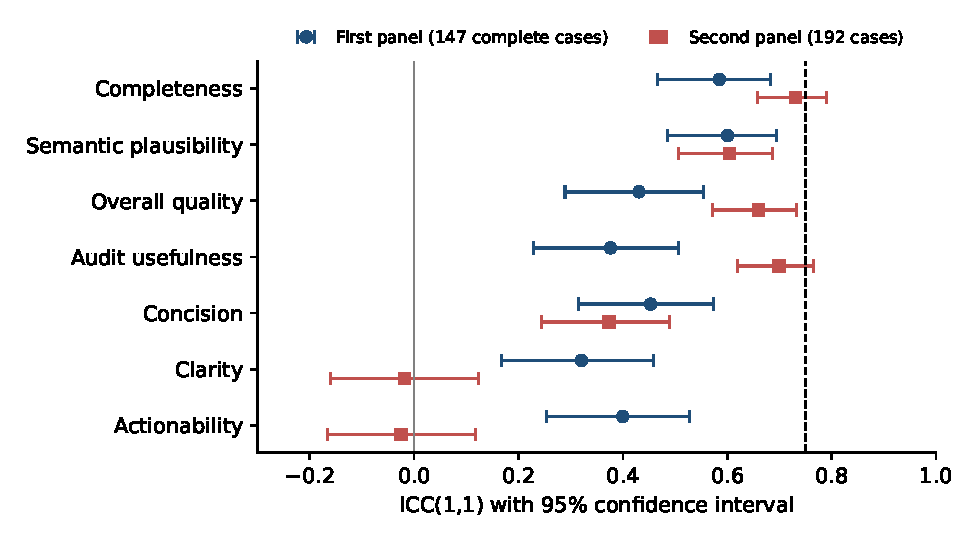
\includegraphics[width=0.85\linewidth]{figures/fig1}
\caption{ICC(1,1) among three LLM judges per dimension, with 95\% confidence
intervals, in the two panels. The dashed line is the 0.75 threshold of good
reliability.}
\label{fig:icc}
\end{figure}

The order of the dimensions was not the same in the two panels. Completeness and
semantic plausibility were among the highest in both. Audit usefulness moved from
0.376 to
0.699 and overall quality from
0.431 to 0.660.
Clarity and actionability fell to about zero. For actionability this is a floor effect:
86\% of the scores of the primary condition
were 1, so there was almost no variation between cases to agree on. For clarity, one
judge hardly varied its score (standard deviation
0.38) and scored on average
0.64 points below the other two, and the
one-way coefficient counts that offset as disagreement.

\subsection{Rubric wording, aggregation and repetition}

Table~\ref{tab:views} gives the ICC of the second panel under the other three views.
Stating the label left agreement almost unchanged. The alternative rubric moved it in
both directions: concision rose from 0.360 to
0.650, clarity fell from 0.026
to $-$0.249, and completeness reached
0.753, above the threshold. In the pooled view
2 dimensions exceeded 0.75, completeness
(0.839) and audit usefulness
(0.820): averaging nine scores removes the
variation between repeated calls and raises the coefficient.

\begin{table}[t]
\centering
\caption{ICC(1,1) of the second panel under three other views
(192 cases). Pooled: the nine scores of a judge for a case (three
conditions, three replicates) are averaged before the coefficient is computed.}
\label{tab:views}
\small
\begin{tabular}{lccc}
\toprule
Dimension & Label stated & Alternative rubric & Pooled \\
\midrule
Completeness & 0.744 & 0.753 & 0.839 \\
Semantic plausibility & 0.594 & 0.566 & 0.664 \\
Overall quality & 0.624 & 0.614 & 0.706 \\
Audit usefulness & 0.730 & 0.668 & 0.820 \\
Concision & 0.360 & 0.650 & 0.524 \\
Clarity & 0.026 & $-$0.249 & $-$0.090 \\
Actionability & $-$0.074 & 0.056 & 0.039 \\
\bottomrule
\end{tabular}
\end{table}

The scores themselves moved little when the label was stated: the largest mean
difference over judges and dimensions was 0.14 points.
Because the primary condition already allowed the label to be derived, this comparison
does not show that the judges ignore the label. The alternative rubric moved the scores
more, by up to 0.50 points (median over judges and
dimensions 0.12).

Repeated calls with temperature 0 did not always return the same score
(Table~\ref{tab:retest}). One judge gave the same score in the three replicates in
93\% to 99\% of the
cases, depending on the dimension; the other two in
65\% to 91\% and in
33\% to 87\%.

\begin{table}[t]
\centering
\caption{Test-retest agreement of the second panel in the primary condition: share of
the 192 cases with the same score in the three replicates, per judge
and dimension.}
\label{tab:retest}
\small
\begin{tabular}{lccc}
\toprule
Dimension & Claude Haiku 4.5 & Gemini 3.8 Flash & GPT-5.4 mini \\
\midrule
Completeness & 0.98 & 0.85 & 0.74 \\
Semantic plausibility & 0.97 & 0.65 & 0.57 \\
Overall quality & 0.98 & 0.83 & 0.59 \\
Audit usefulness & 0.99 & 0.73 & 0.61 \\
Concision & 0.93 & 0.79 & 0.33 \\
Clarity & 0.96 & 0.68 & 0.47 \\
Actionability & 0.97 & 0.91 & 0.87 \\
\bottomrule
\end{tabular}
\end{table}

\subsection{Scores and the technical metrics}

Table~\ref{tab:metrics} gives the correlation between the overall-quality score and each
technical metric within each explainer. The score rose with fidelity for the four
explainers (Spearman correlation from 0.35
to 0.59), in all four after Holm's
correction. Of the other 16 correlations two remained after the correction: stability
for Anchors (0.42) and sparsity
for LIME (0.73). In the regression
with explainer and dataset as strata the rank of the score rose with the rank of
fidelity (slope 0.27, adjusted
$p$ $<$0.001), of faithfulness gap, of sparsity and of
stability, and not with runtime (adjusted $p =$ 0.237).

\begin{table}[t]
\centering
\caption{Spearman correlation between the overall-quality score (second panel, primary
condition, mean of judges and replicates) and the technical metrics, within each
explainer. An asterisk marks $p < 0.05$ after Holm's correction over the 20 tests.}
\label{tab:metrics}
\small
\begin{tabular}{lccccc}
\toprule
Explainer (cases) & Fidelity & Stability & Sparsity & Faithfulness gap & Runtime \\
\midrule
Anchors (76) & 0.35* & 0.42* & $-$0.19 & 0.30 & $-$0.27 \\
SHAP (52) & 0.49* & 0.26 & $-$0.05 & $-$0.10 & 0.14 \\
LIME (32) & 0.59* & $-$0.03 & 0.73* & 0.17 & 0.21 \\
DiCE (32) & 0.58* & 0.18 & 0.31 & 0.31 & 0.31 \\
\bottomrule
\end{tabular}
\end{table}

Because the metrics were printed in the prompt, this result has a narrow reading: the
overall score of the judges follows the fidelity value they were shown. It does not show
that a judge can tell a faithful explanation from an unfaithful one by reading it.

\section{Discussion}

The answer to the first two questions is negative and it replicates. With the rubric and
the primary prompt, three small LLM judges did not reach good agreement on any of seven
dimensions, in two panels of different models on the same cases. The second panel shows
why a single number should not carry this conclusion: the confidence intervals of two
dimensions cross the threshold, the order of the dimensions changes with the panel, and
two dimensions that had some agreement in the first panel have none in the second.
Agreement is a property of a panel and a rubric together, not of a dimension.

The third question has a practical answer. Three choices that studies rarely report
changed the result. Rewording the rubric moved the ICC of concision by about 0.3 and
that of clarity in the opposite direction. Averaging repeated calls and prompt variants
before computing the coefficient raised two dimensions above the threshold, because the
average hides the variation of a judge with itself. And that variation is not small:
with temperature 0, one judge repeated its score almost always and another in fewer
than half of the cases for some dimensions. A study that uses LLM judges should state
the models, the full rubric, the number of calls per item and the aggregation rule, and
should report the reliability of a single call if single calls are what it uses.

The fourth question cannot be answered fully with these data. The overall score
followed fidelity within every explainer, but fidelity was in the prompt. The finding
still has a consequence: a judge that is given technical metrics may return them in
another form, and then its score adds no independent evidence about meaning. Whether
the judges of this class read anything about faithfulness in the explanation itself
needs a condition without the metrics.

The study has limits. It measures agreement among LLM judges and has no human scores,
so it says nothing about whether the judges are right; a reliable panel could still be
wrong, and an unreliable one cannot be right consistently. Both panels are small,
low-cost models, and the conclusion is limited to that class. The templates and
responses of the first panel were lost, so its condition and aggregation are unknown
and the second run is not a reproduction. No condition withheld the true label, and all
showed the technical metrics. The cases are unbalanced across explainers and datasets,
and LIME and DiCE appear in one dataset only. Actionability had almost no variation.
The analysis of scores against metrics was planned after the runs.

\section{Conclusions}

Three LLM judges did not agree well enough on the quality of post-hoc explanations to
be used as a confirmatory measure: no dimension reached an ICC(1,1) of 0.75 in the
primary condition of either of two panels (highest values
0.601 and 0.731). The threshold was
crossed only with another rubric wording or after averaging repeated calls and prompt
variants, and the order of the dimensions changed with the panel. The overall score
followed the fidelity value shown in the prompt. Scores from LLM judges of this class
are usable as exploratory evidence, with the panel, the rubric and the aggregation
reported; a comparison with human raters and a prompt without technical metrics are the
next steps.

\section*{Data availability}
\iffull
The three datasets are public
\cite{becker1996adult,hofmann1994statlog,wolberg1993breast}. The case inventory, the
rendered prompts, the raw and parsed responses of the second panel, the aggregate tables
of the first panel and the analysis code are available at
\url{https://github.com/jonnabio/xai-eval-framework} (release
\texttt{\papercrelease}), archived at \papercarchive. Every reported value can be
regenerated by following \texttt{docs/reports/paper\_c/README.md}.
\else
The three datasets are public
\cite{becker1996adult,hofmann1994statlog,wolberg1993breast}. The case inventory, the
rendered prompts, the raw and parsed responses of the second panel, the aggregate tables
of the first panel and the analysis code are in a public repository and a versioned
archive, with instructions to regenerate every reported value; their addresses are
withheld for double-blind review.
\fi

\bibliographystyle{IEEEtran}
\bibliography{references}

% Journal AI policy: state the tools, the purpose and how the results were verified;
% placed after the references, as in the journal's published articles. Same statement as
% Paper D (author decision, 2026-10-04). The LLMs used as judges are the object of the
% study and are described in the methods.
\section*{Declaration on the Use of Artificial Intelligence (AI)}
The author declares the use of the AI tool Claude (Anthropic), under the author's
direction, to help write the analysis and figure code, edit the English text, translate the
abstract into Spanish and format the references. The research questions, analysis plan,
design and interpretation are the author's. All contents were thoroughly reviewed by the
author to ensure accuracy and coherence. The language models used as judges are the object
of the study and are described in the methods.

\end{document}
